% =====================================================================
%  04 模型的建立与求解(建模手写模型,编程手写求解数值,论文手润色)
%  每个问题一个小节:建模思路 → 符号定义 → 公式推导 → 求解/算法。
%  数值占位符:\textbf{(待回填:……)} 由编程手跑完脚本后回填。
% =====================================================================
\section{模型的建立与求解}

\subsection{问题一:残损存在性分类模型的建立与求解}

\subsubsection{建模思路}

问题一是二分类任务:给定图像 $I$,判断其是否含有残损。由于训练集中不存在“无残损”样本,直接训练有监督的二分类器不可行(分类器只会退化到“恒判有残损”),因此我们将“是否存在残损”归约为“能否检测出残损区域”,把问题一与问题二的残损检测统一到同一框架之下。

\subsubsection{检测归约的存在性分类模型}

设残损检测模型为 $D(\cdot)$(问题二建立),对图像 $I$ 输出候选框集合
\[
\mathcal{B}=D(I)=\{(b_i,c_i,s_i)\}_{i=1}^{K},
\]
其中 $b_i=(x_i,y_i,w_i,h_i)$ 为框位置,$c_i$ 为类别,$s_i\in[0,1]$ 为置信度。此处 $D(\cdot)$ 取 NMS 后、top-4 截断前的全部候选框:每图至多 4 框的截断仅作用于提交与问题三的 top-4 口径,不压缩问题一的存在性判定依据。定义置信度不低于阈值 $\tau$ 的检测框个数为
\[
N(I;\tau)=\bigl|\{(b_i,c_i,s_i)\in D(I):s_i\ge\tau\}\bigr|.
\]
则问题一的存在性分类函数为
\[
f(I)=\mathbf{1}\{N(I;\tau)\ge 1\}
=\begin{cases}1, & N(I;\tau)\ge 1,\\ 0, & N(I;\tau)=0.\end{cases}
\]
其含义是:若图像中至少存在一个置信度不低于 $\tau$ 的残损检测框,则判定“存在残损”,否则判定“无残损”。该归约成立的核心前提是\textbf{检测器对无残损图像输出低置信度候选框}:一方面,单阶段检测器在训练中将大量未匹配真实目标的网格单元赋为背景标签,分类分支被训练为对背景区域输出低得分,天然具备一定的背景判别能力;另一方面,该前提并非先验成立,将由合成负样本上的低假阳率实证检验(见求解结果)。据此,无需真实负样本图像即可完成存在性判断。

\subsubsection{阈值 $\tau$ 的选择}

阈值 $\tau$ 是关键超参。为避免“在同一数据集上既选阈值又报告指标”造成的乐观偏差,将合成负样本划分为调参半与评估半:在\textbf{调参集}(330 张训练期验证正样本 + 调参半合成负样本,330 张与问题二的训练期验证划分一致)上通过最大化 $F_1$ 选取
\[
\tau^{*}=\arg\max_{\tau}\, F_1(\tau),
\]
最终分类指标在与调参隔离的\textbf{评估集}(413 张验证正样本 + 评估半合成负样本)上报告。

\subsubsection{评价指标}

以“存在残损”为正类,记 $TP/FP/TN/FN$ 分别为真阳、假阳、真阴、假阴,定义
\[
Acc=\frac{TP+TN}{TP+FP+TN+FN},\quad
P=\frac{TP}{TP+FP},\quad
R=\frac{TP}{TP+FN},\quad
F_1=\frac{2PR}{P+R},
\]
并绘制 ROC 曲线计算 $AUC$。由于训练集与验证集均无“无残损”图像,无法直接获得真实负样本,故合成负样本:从残损图像中裁取不含任何标注框的区域(裁剪窗口避开标注框并外扩边距,以降低框外残损混入的风险),随机拼合为 $640\times640$ 整图,并抽检剔除拼接伪影(“不含标注框”不等于“不含残损”,锈蚀扩散与漏标等情形以人工抽检把关)。合成负样本集划分为调参半与评估半,分别与 330 张训练期验证正样本、413 张验证正样本构成调参集与评估集,二者相互隔离。ROC 曲线以图像级最高置信度
\[
S(I)=\max_{(b_i,c_i,s_i)\in D(I)} s_i
\]
(图像无检测框时记 $S(I)=0$)作为连续得分绘制。

\subsubsection{模型求解}

求解流程为:训练检测器 $D(\cdot)$ → 合成负样本并划分为调参半/评估半 → 在调参集上扫描 $\tau$ 求最优阈值 $\tau^{*}$ → 在评估集上输出分类结果与指标。

\subsubsection{求解结果}

调参集(330 张训练期验证正样本 + $\textbf{(待回填:……)}$ 张调参半合成负样本)上求得最优阈值 $\tau^{*}=\textbf{(待回填:……)}$;在与调参隔离的评估集(413 张验证正样本 + $\textbf{(待回填:……)}$ 张评估半合成负样本)上的分类指标见表~\ref{tab:q1-cls},ROC 曲线与 $F_1(\tau)$ 曲线见图~\ref{fig:q1-metrics}。结果表明\textbf{(待回填:一句结论)}。

% 待新增表 tab:q1-cls(取消注释,数值逐个替换 0.xxxx):
% \begin{table}[h]
% \centering
% \caption{问题一分类结果(评估集,与调参集隔离)}
% \label{tab:q1-cls}
% \begin{tabular}{ccccc}
% \toprule
% Acc & P & R & $F_1$ & AUC \\
% \midrule
% 0.xxxx & 0.xxxx & 0.xxxx & 0.xxxx & 0.xxxx \\
% \bottomrule
% \end{tabular}
% \end{table}
%
% 待新增图 fig:q1-metrics(取消注释;由 fig_q1_metrics.py 生成):
% \begin{figure}[h]
% \centering
% 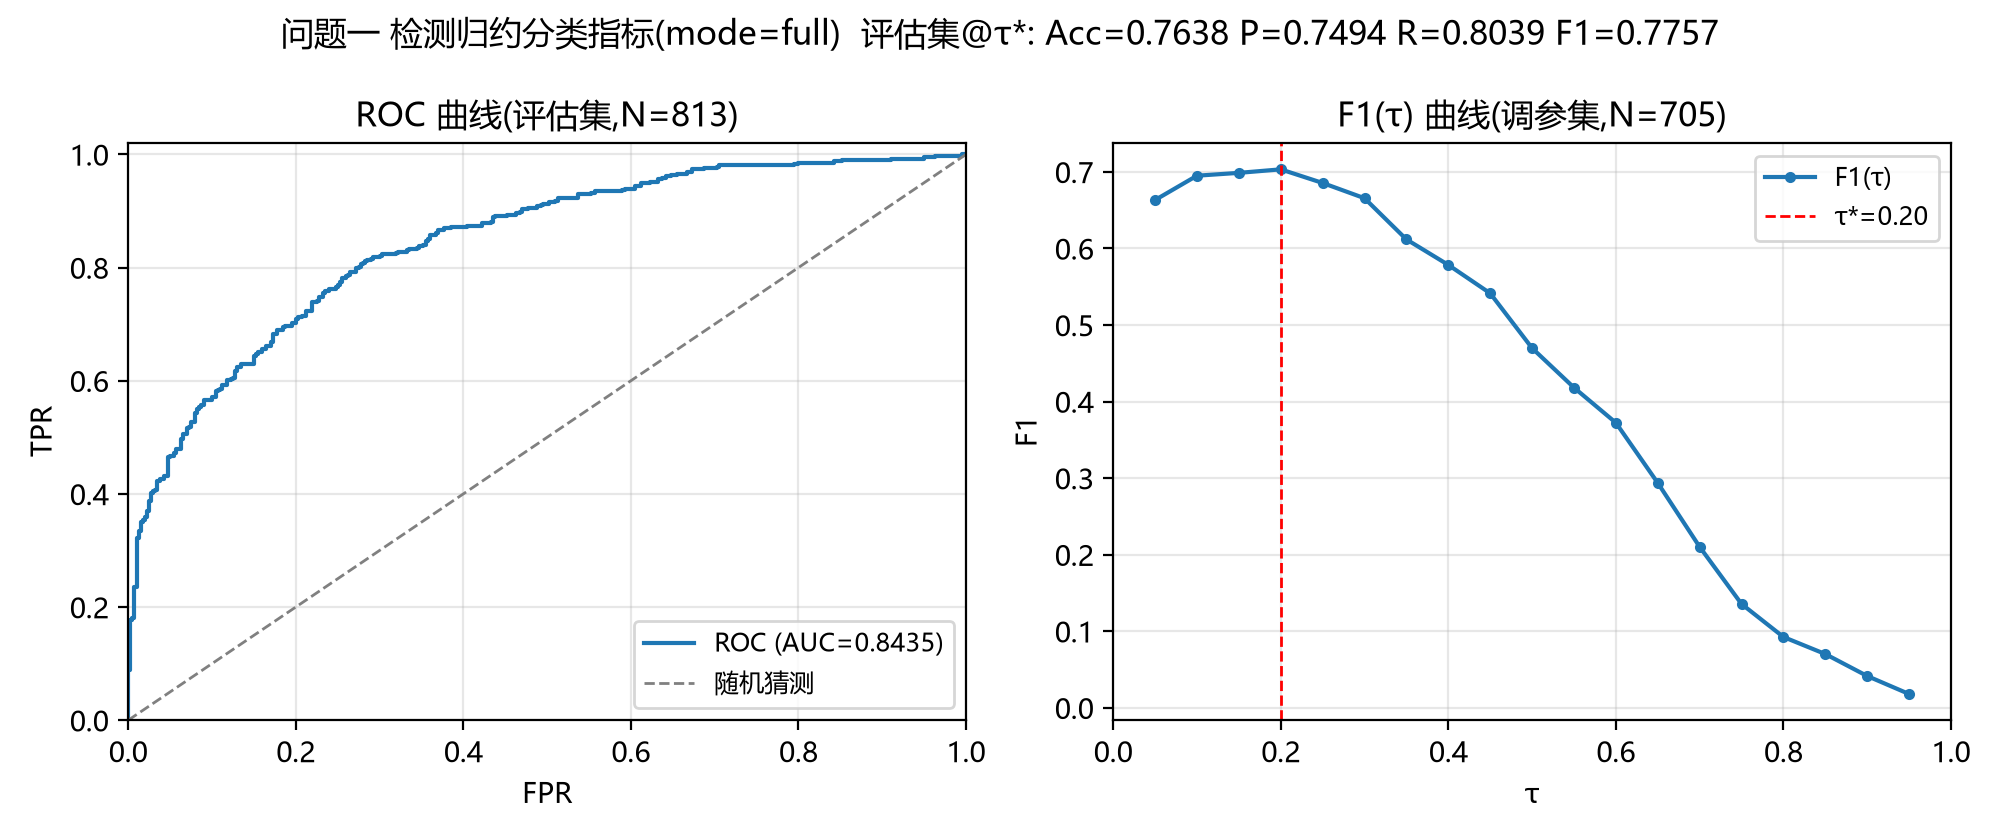
\includegraphics[width=0.95\textwidth]{figures/fig_q1_metrics.png}
% \caption{问题一 ROC 曲线(左,评估集)与 $F_1(\tau)$ 曲线(右,调参集,标注 $\tau^{*}$)}
% \label{fig:q1-metrics}
% \end{figure}

\subsection{问题二:残损检测与分割模型的建立与求解}

\subsubsection{建模思路}

问题二要求定位残损位置并识别类别,同时输出像素级分割,本质是\textbf{目标检测 + 实例分割}的多任务问题。考虑到港口场景对实时性、多尺度与小目标的需求,选用\textbf{单阶段实例分割网络 YOLOv8-seg}作为统一框架:其以卷积神经网络(CNN)主干提取多尺度特征,经特征金字塔融合,由解耦检测头一次前向同时输出边界框、类别与掩码,实现端到端的检测与分割。

\subsubsection{网络结构}

网络由主干(Backbone)、颈部(Neck)与检测头(Head)三部分组成:

\begin{itemize}
\item \textbf{主干}:采用卷积神经网络 CSPDarknet(由 C2f 模块堆叠的 CNN),通过逐层卷积与下采样输出 $P_3,P_4,P_5$ 三个尺度的特征图,分别对应小、中、大目标;
\item \textbf{颈部}:采用 FPN + PAN 结构,自顶向下与自底向上双向融合多尺度特征,增强小目标特征表达;
\item \textbf{检测头}:解耦为三个分支——分类分支输出类别得分,回归分支输出边界框(采用 anchor-free 方式直接回归中心点与宽高),分割分支输出掩码原型与掩码系数,两者线性组合得到实例掩码。
\end{itemize}

\subsubsection{边界框回归}

采用 anchor-free 的编码方式:对特征图每个网格单元直接预测归一化中心点偏移与宽高 $(x_c,y_c,w,h)$,并以完整交并比(CIoU)作为回归目标,兼顾重叠度、中心点距离与长宽比一致性。

\subsubsection{损失函数}

总损失由分类、回归、分割三项加权构成:
\[
\mathcal{L}=\lambda_{cls}\mathcal{L}_{cls}+\lambda_{box}\mathcal{L}_{box}+\lambda_{seg}\mathcal{L}_{seg}.
\]
其中:
\begin{itemize}
\item \textbf{分类损失} $\mathcal{L}_{cls}$ 采用二值交叉熵(BCE),针对类别不平衡,可进一步用类别加权或 Varifocal 损失;
\item \textbf{回归损失} $\mathcal{L}_{box}$ 采用 CIoU 损失与分布聚焦损失(DFL)的组合;
\item \textbf{分割损失} $\mathcal{L}_{seg}$ 采用 Dice 损失与二值交叉熵的组合:
\[
\mathcal{L}_{seg}=1-\frac{2\sum_i \hat{m}_i m_i}{\sum_i \hat{m}_i+\sum_i m_i+\varepsilon},
\]
其中 $\hat{m}_i$ 为掩码像素预测值,$m_i$ 为像素真值,$\varepsilon$ 为防止除零的小常数。
\end{itemize}

\subsubsection{小目标与多尺度处理}

针对数据集中大量小尺度残损,采取三方面措施:提高输入分辨率(由 $640$ 放大至 $1280$)——放大虽不引入新的图像细节,但使小目标在特征金字塔下采样后保留更多有效像素,缓解其在深层特征上的过度压缩;在颈部引入更浅层的特征层($P_2$)以增强小目标响应;训练时采用多尺度训练与马赛克等数据增强,提升尺度鲁棒性。

\subsubsection{后处理:非极大值抑制与 top-4 筛选}

检测头输出大量候选框,需经非极大值抑制(NMS)去除同一目标的重复框:按置信度降序排列,保留置信度最高者,并抑制与其 IoU 超过 $\tau_{nms}$ 的候选框。考虑到评测约定每图最多取 4 个残损(按严重程度),而官方未给出严重度的具体定义,本文以边界框面积作为严重度代理(面积越大越严重),定义
\[
sev(b_i)=w_i\,h_i,
\]
NMS 后按 $sev(b_i)$ 降序取前 4 个作为最终输出;面积与置信度两种排序方式对最终指标的影响将在问题三作灵敏度分析。

\subsubsection{评价指标}

\textbf{检测指标}:以 IoU 阈值判定正样本,定义查准率 $P$ 与召回率 $R$,平均精度为 PR 曲线下面积
\[
AP=\int_0^1 P(R)\,\mathrm{d}R,
\]
对所有类别取平均得均值平均精度 $mAP$;常用 $mAP@0.5$ 与 $mAP@0.5:0.95$ 两个口径,并按目标尺度报告小/中/大目标 $AP$。本章检测指标按\textbf{全框口径}报告,以反映模型完整检测能力;评测要求的“每图最多 4 框”口径在问题三的 top-4 对比实验(表~\ref{tab:q3-top4})中单独考察。另报告分类混淆矩阵(含背景行/列),统计各真实类别的实例被判定为何类别,以考察三类残损间的混淆以及漏检、误检情况。

\textbf{分割指标}:对类别 $c$,预测掩码 $\hat{M}_c$ 与真实掩码 $M_c$ 的 Dice 系数与平均交并比分别为
\[
\mathrm{Dice}=\frac{2|\hat{M}_c\cap M_c|}{|\hat{M}_c|+|M_c|},\qquad
\mathrm{mIoU}=\frac{1}{C}\sum_{c}\frac{|\hat{M}_c\cap M_c|}{|\hat{M}_c\cup M_c|}.
\]

\subsubsection{模型求解}

求解流程为:构建 YOLOv8-seg 训练管线 → 数据增强与类别加权 → 训练与验证 → NMS 与 top-4 后处理 → 输出检测与分割指标。

\subsubsection{求解结果}

(待编程手回填数值与图。)检测结果见表~\ref{tab:q2-det},分割结果见表~\ref{tab:q2-seg},训练收敛曲线、各类 PR 曲线、混淆矩阵与可视化样例分别见图~\ref{fig:q2-loss}、图~\ref{fig:q2-pr}、图~\ref{fig:q2-confusion}、图~\ref{fig:q2-visual}。结果表明\textbf{(待回填:一句结论)}。

% 待新增表 tab:q2-det(取消注释,数值逐个替换 0.xxxx):
% \begin{table}[h]
% \centering
% \caption{问题二检测结果(验证集)}
% \label{tab:q2-det}
% \begin{tabular}{lccc}
% \toprule
% 类别 & AP@0.5 & AP@0.5:0.95 & 训练集实例数 \\
% \midrule
% Dent(凹陷)  & 0.xxxx & 0.xxxx & 3934 \\
% Hole(破洞)  & 0.xxxx & 0.xxxx & 946 \\
% Rusty(锈蚀) & 0.xxxx & 0.xxxx & 3158 \\
% \midrule
% 总体 mAP    & 0.xxxx & 0.xxxx & — \\
% \bottomrule
% \end{tabular}
% \end{table}
%
% 待新增表 tab:q2-seg(取消注释,数值逐个替换 0.xxxx):
% \begin{table}[h]
% \centering
% \caption{问题二分割结果(验证集)}
% \label{tab:q2-seg}
% \begin{tabular}{lcc}
% \toprule
% 类别 & Dice & mIoU \\
% \midrule
% Dent(凹陷)  & 0.xxxx & 0.xxxx \\
% Hole(破洞)  & 0.xxxx & 0.xxxx \\
% Rusty(锈蚀) & 0.xxxx & 0.xxxx \\
% \midrule
% 总体 & 0.xxxx & 0.xxxx \\
% \bottomrule
% \end{tabular}
% \end{table}
%
% 待新增图 fig:q2-loss / fig:q2-pr / fig:q2-confusion / fig:q2-visual(取消注释;由对应 fig_*.py 生成):
% \begin{figure}[h]
% \centering
% 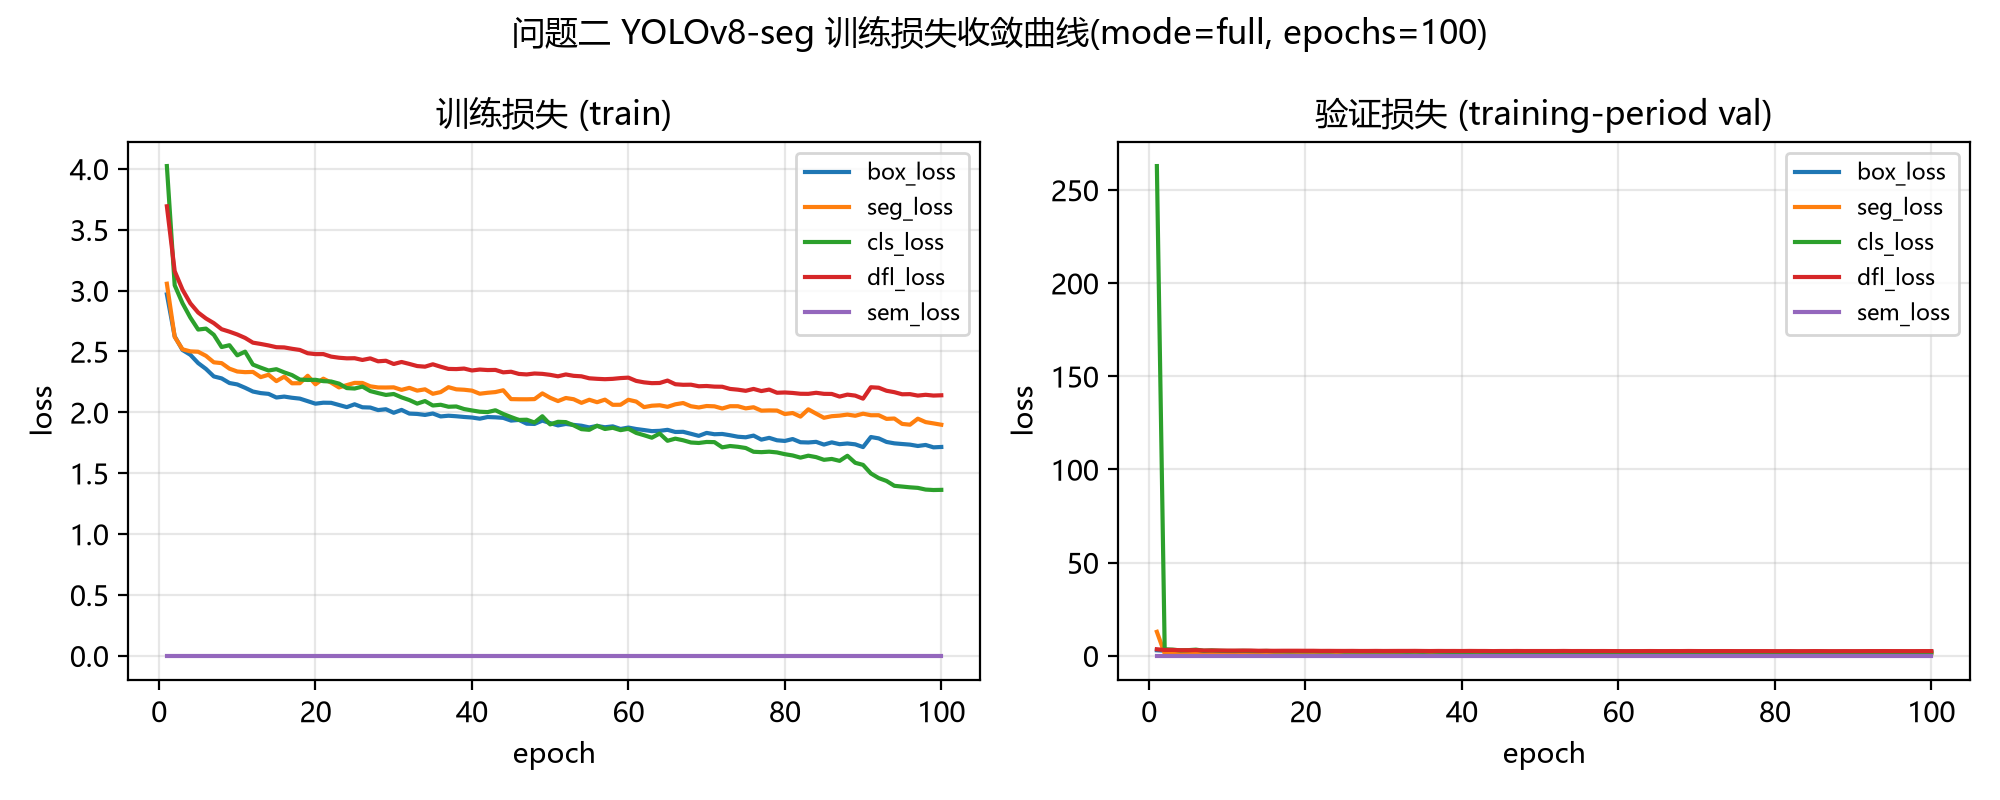
\includegraphics[width=0.85\textwidth]{figures/fig_q2_loss.png}
% \caption{训练损失收敛曲线}
% \label{fig:q2-loss}
% \end{figure}
% \begin{figure}[h]
% \centering
% 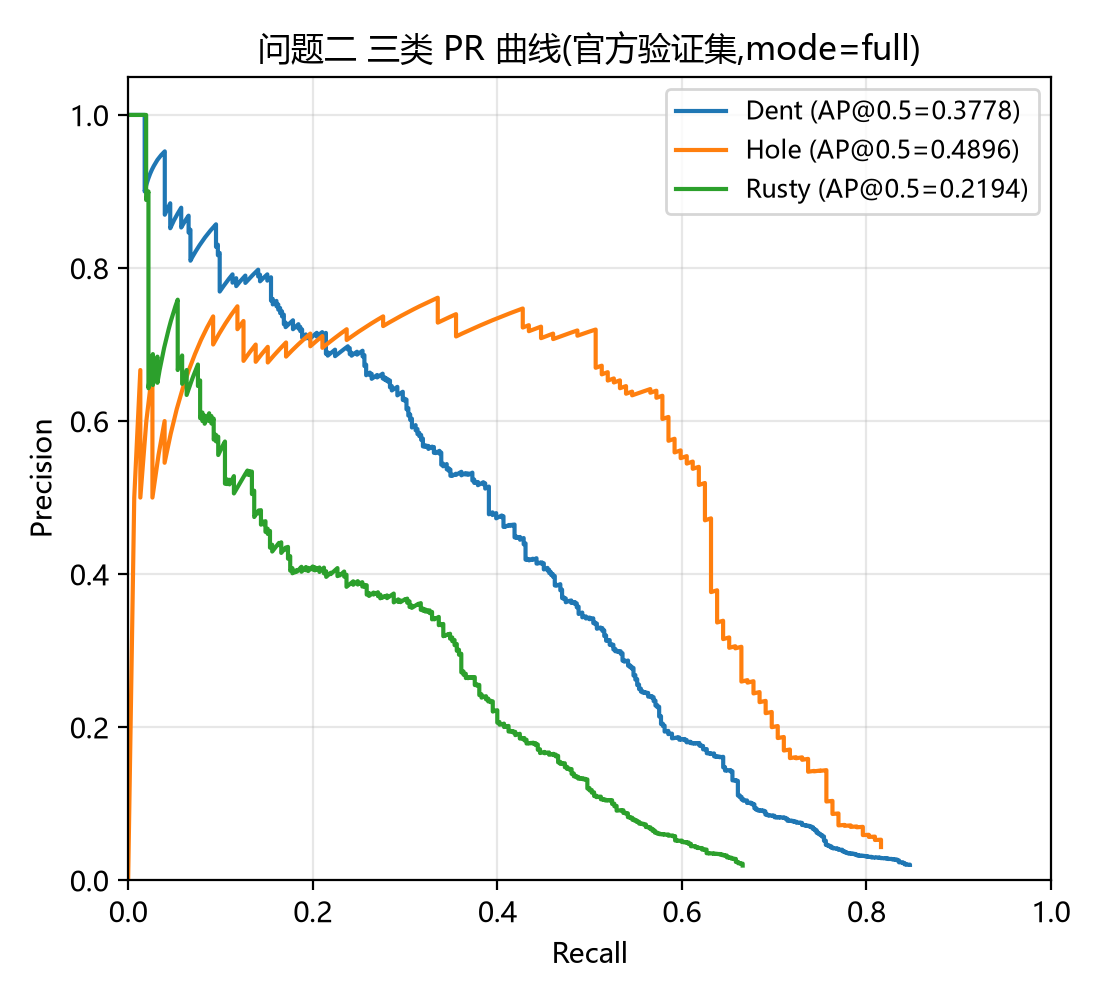
\includegraphics[width=0.85\textwidth]{figures/fig_q2_pr.png}
% \caption{三类残损的 PR 曲线}
% \label{fig:q2-pr}
% \end{figure}
% \begin{figure}[h]
% \centering
% 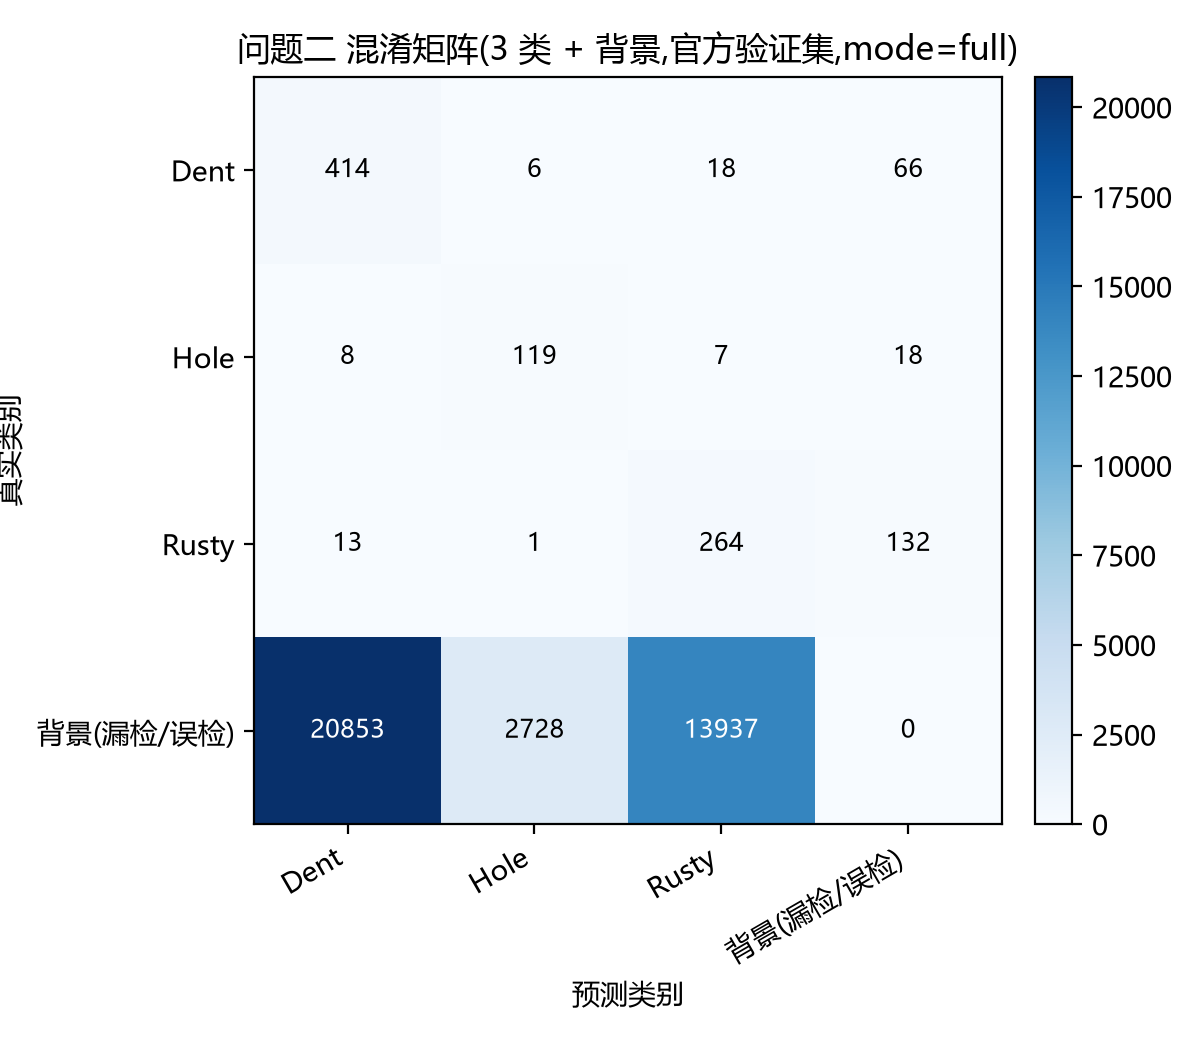
\includegraphics[width=0.6\textwidth]{figures/fig_q2_confusion.png}
% \caption{分类混淆矩阵(3 类 + 背景,含漏检/误检行列)}
% \label{fig:q2-confusion}
% \end{figure}
% \begin{figure}[h]
% \centering
% 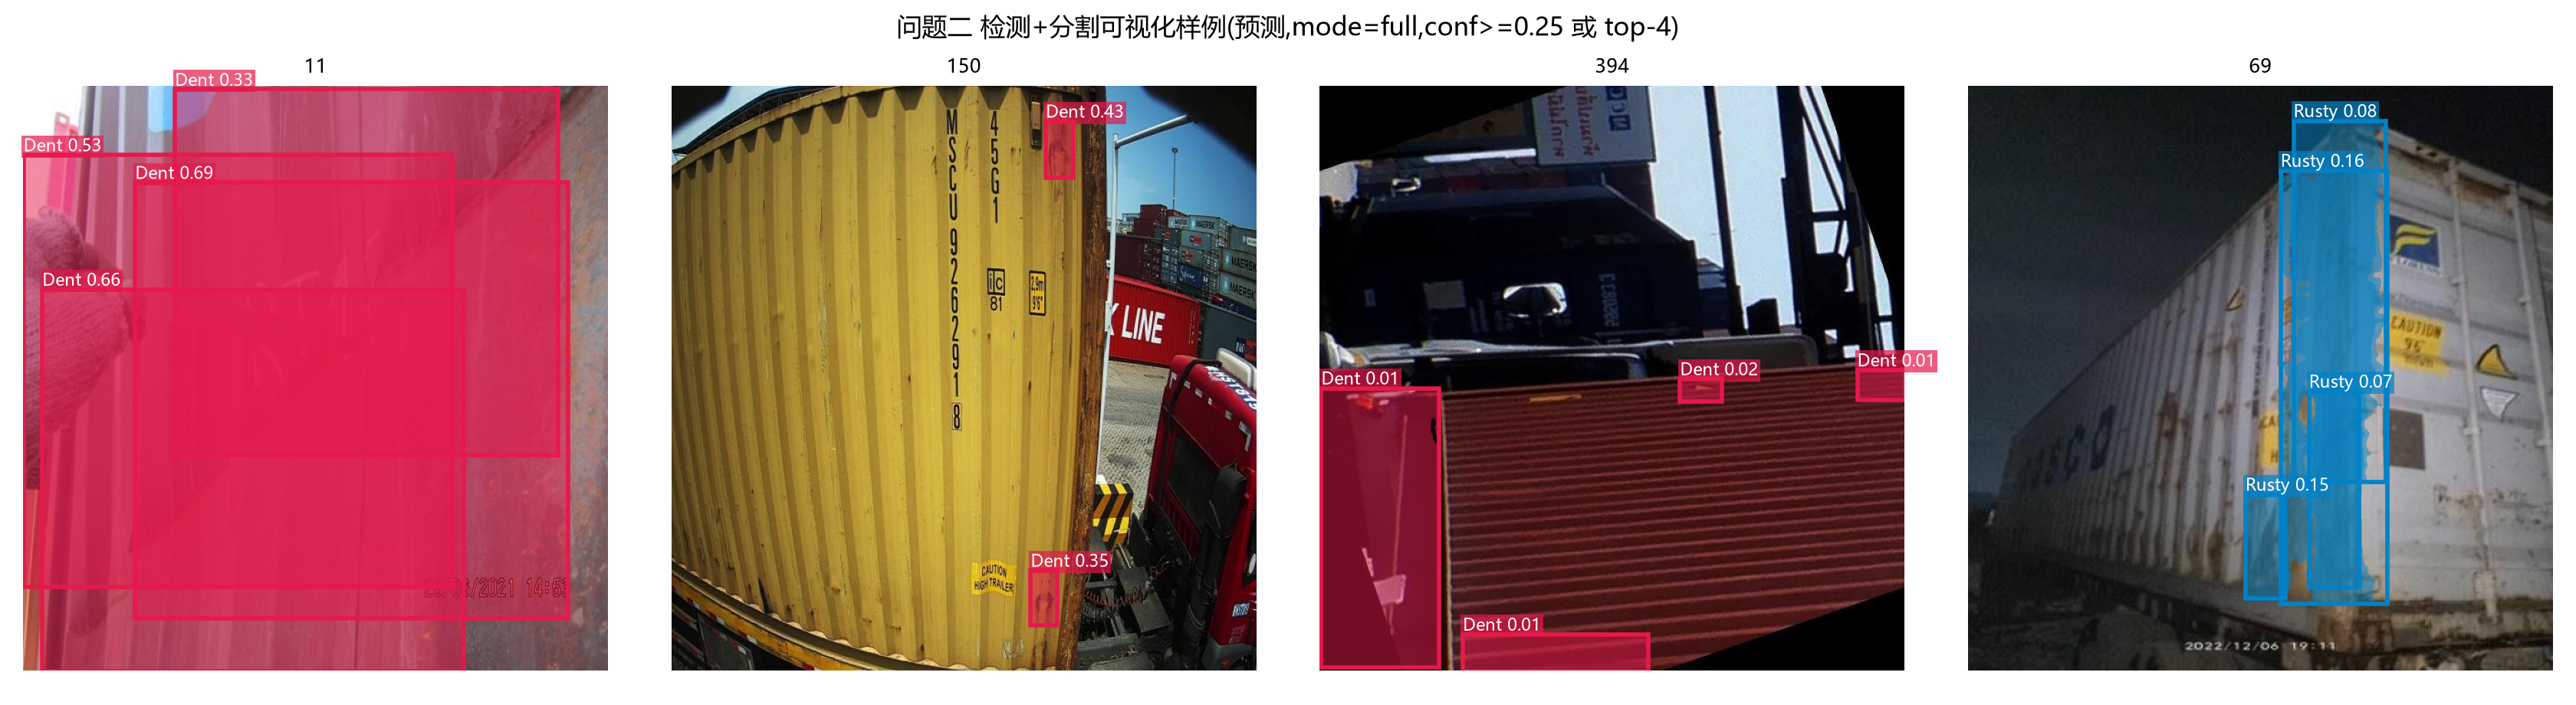
\includegraphics[width=0.9\textwidth]{figures/fig_q2_visual.png}
% \caption{检测与分割可视化样例(框=检测,彩色区域=分割掩码)}
% \label{fig:q2-visual}
% \end{figure}

\subsection{问题三:多维度评估体系的建立与求解}

\subsubsection{建模思路}

问题三要求对问题一、问题二建立的模型从不同维度进行评估。为此,建立“四维评估 + 对比消融 + 灵敏度”的评估体系:从准确性、鲁棒性、效率、可解释性四个维度检验模型,再以对比实验与消融实验支撑模型选择的合理性,最后对关键超参作灵敏度分析。

\subsubsection{准确性评估}

分类指标 $Acc,P,R,F_1$ 已在问题一给出,此处补充 $AUC$:以问题一定义的图像级得分 $S(I)$ 为决策变量,对其阈值作全范围扫描得到 ROC 曲线(横轴为假阳率 $FPR$、纵轴为真阳率 $TPR$),曲线下面积即
\[
AUC=\int_0^1 TPR\,\mathrm{d}FPR,
\]
其中 $TPR$ 为真阳率、$FPR$ 为假阳率。检测指标沿用问题二的 $mAP@0.5$ 与 $mAP@0.5:0.95$,并按目标面积划分为小、中、大目标分别报告 $AP_s,AP_m,AP_l$,以检验模型的多尺度能力;分割指标沿用 $mIoU$ 与 $Dice$。

\subsubsection{鲁棒性评估}

针对复杂背景与多变光照,构造扰动测试集:对验证集分别施加亮度缩放($\times0.7/1.3$)、对比度调整、高斯噪声与高斯模糊,模拟光照变化、雨水与污渍干扰。对第 $j$ 项指标,定义扰动下的性能衰减率
\[
\Delta_j=\frac{y_j^{clean}-y_j^{pert}}{y_j^{clean}}\times 100\%,
\]
其中 $y_j^{clean},y_j^{pert}$ 分别为干净与扰动条件下第 $j$ 项指标的取值;$\Delta_j$ 越小,模型鲁棒性越强。

\subsubsection{效率评估}

港口场景对实时性有要求,以单张图像平均推理耗时 $t_{inf}$ 计算帧率
\[
FPS=\frac{1}{t_{inf}},
\]
并结合参数量、显存占用评估部署可行性;推理条件(硬件、批量、输入分辨率)保持一致并在结果表~\ref{tab:q3-eff} 中注明。

\subsubsection{可解释性评估}

用 Grad-CAM 可视化模型决策依据:对类别 $c$ 的得分 $y^c$,第 $k$ 个特征图 $A^k$ 的权重为
\[
\alpha_k^c=\frac{1}{Z}\sum_{i,j}\frac{\partial y^c}{\partial A^k_{ij}},
\]
类别激活图为
\[
G^c=\mathrm{ReLU}\Bigl(\sum_k \alpha_k^c A^k\Bigr).
\]
若激活区集中于残损区域而非背景,则表明模型学到的是残损本身的可判别特征。

\subsubsection{对比实验}

设计两组对比:(1) 问题一方案对比——检测归约方案与自建小 CNN 分类器、传统特征 + SVM 基线对比。为隔离训练与评估,自建分类器以训练正样本 + 调参半合成负样本训练,三方案统一在问题一的评估集(413 张验证正样本 + 评估半合成负样本)上评估,训练/调参数据与评估数据不重叠,保证比较公平。合成负样本由 4 块 clean cell 拼接而成,接缝等结构痕迹可能构成可被分类器利用的捷径信号;为排除其对结论的影响,另收集 43 张真实无残损集装箱照片(不拼接)作方向性诊断——三方案不重新训练、沿用各自选定的阈值,在真实负样本口径下复评 $AUC$,检验合成口径结论的稳健性。由于真实负样本取景尺度与训练分布不完全一致、样本量偏小,该口径仅作方向性诊断,不作正式基准;(2) 问题二模型对比——不同骨干规模(YOLOv8n/s/m-seg)的精度—效率权衡。

\subsubsection{消融实验}

对问题二模型的关键设计作\textbf{逐项累加式消融}:自基准配置(无类别加权/无 $P_2$/$640$ 输入/无强增强)起依次加入类别加权损失、$P_2$ 小目标检测头、高分辨率输入($1280$)、强数据增强,逐行考察各模块对 $mAP$ 与 $AP_s$ 的贡献。为控制训练成本,消融各配置统一训练 30 epoch,仅用于比较模块间的相对增量;最终模型的绝对指标见问题二结果(100 epoch 训练),两者口径不同,不可直接对比。

\subsubsection{灵敏度分析}

对关键超参扫描分析:(1) 置信度阈值 $\tau$——扫描 $\tau$ 绘制 $F_1(\tau)$ 曲线,验证问题一的最优阈值选择;(2) NMS 阈值 $\tau_{nms}$;(3) top-4 排序方式——按面积(严重度代理)与按置信度两种排序对 $mAP$ 的影响;(4) 输入分辨率 $640/960/1280$ 对精度与速度的权衡。

\subsubsection{模型求解}

求解流程为:在验证集上输出四维评估指标 → 扰动鲁棒性测试 → 对比与消融实验 → 超参灵敏度扫描。

\subsubsection{求解结果}

(待编程手回填数值与图。)鲁棒性衰减见表~\ref{tab:q3-robust}、图~\ref{fig:q3-robust};对比实验结果见表~\ref{tab:q3-compare}(问题一方案以合成/真实负样本双口径 $AUC$ 报告);效率对比见表~\ref{tab:q3-eff};消融结果见表~\ref{tab:q3-ablation}(各配置 30 epoch,仅比较相对增量);top-4 排序方式对比见表~\ref{tab:q3-top4};超参灵敏度曲线见图~\ref{fig:q3-sens};Grad-CAM 可视化见图~\ref{fig:q3-gradcam}。结果表明\textbf{(待回填:一句结论)}。

% 待新增表 tab:q3-robust(取消注释,数值逐个替换 0.xxxx / x.xx):
% \begin{table}[h]
% \centering
% \caption{扰动鲁棒性评估(验证集)}
% \label{tab:q3-robust}
% \begin{tabular}{lccc}
% \toprule
% 扰动 & mAP@0.5 & $\Delta_j$(\%) & $F_1$ \\
% \midrule
% 无扰动(基准) & 0.xxxx & — & 0.xxxx \\
% 亮度 $\times0.7$   & 0.xxxx & x.xx & 0.xxxx \\
% 亮度 $\times1.3$   & 0.xxxx & x.xx & 0.xxxx \\
% 对比度调整 & 0.xxxx & x.xx & 0.xxxx \\
% 高斯噪声   & 0.xxxx & x.xx & 0.xxxx \\
% 高斯模糊   & 0.xxxx & x.xx & 0.xxxx \\
% \bottomrule
% \end{tabular}
% \end{table}
%
% 待新增表 tab:q3-compare(取消注释,数值逐个替换 0.xxxx;问题一以双口径 AUC 报告,数值见 code/src/noted.md 第 4.3 节):
% \begin{table}[h]
% \centering
% \caption{对比实验结果(验证集;问题一为合成/真实负样本双口径 $AUC$)}
% \label{tab:q3-compare}
% \begin{tabular}{lccc}
% \toprule
% 方案 & $AUC$(合成负样本) & $AUC$(真实负样本, $N=43$) & mAP@0.5 \\
% \midrule
% 问题一:传统特征+SVM(合成负样本训练) & 0.xxxx & 0.xxxx & — \\
% 问题一:自建小 CNN(合成负样本训练)   & 0.xxxx & 0.xxxx & — \\
% 问题一:检测归约(本文)               & 0.xxxx & 0.xxxx & — \\
% \midrule
% 问题二:YOLOv8n-seg & — & — & 0.xxxx \\
% 问题二:YOLOv8s-seg(本文) & — & — & 0.xxxx \\
% 问题二:YOLOv8m-seg & — & — & 0.xxxx \\
% \bottomrule
% \end{tabular}
% \end{table}
%
% 待新增表 tab:q3-eff(取消注释,数值逐个替换 0.xxxx):
% \begin{table}[h]
% \centering
% \caption{问题二模型效率对比(统一硬件,batch=1,输入 1280)}
% \label{tab:q3-eff}
% \begin{tabular}{lccc}
% \toprule
% 模型 & 参数量(M) & FPS & mAP@0.5 \\
% \midrule
% YOLOv8n-seg & 0.xxxx & 0.xxxx & 0.xxxx \\
% YOLOv8s-seg(本文) & 0.xxxx & 0.xxxx & 0.xxxx \\
% YOLOv8m-seg & 0.xxxx & 0.xxxx & 0.xxxx \\
% \bottomrule
% \end{tabular}
% \end{table}
%
% 待新增表 tab:q3-ablation(取消注释,数值逐个替换 0.xxxx;数值见 code/src/noted_q3.md 第 2 节):
% \begin{table}[h]
% \centering
% \caption{问题二模型消融实验(逐项累加:每行在前一行基础上新增一项;各配置统一训练 30 epoch,仅用于比较相对增量,与主结果表的 100 epoch 口径不可直接对比)}
% \label{tab:q3-ablation}
% \begin{tabular}{lcc}
% \toprule
% 配置 & mAP@0.5 & $AP_s$ \\
% \midrule
% 基准(无类别加权/无 P2/640 输入/无强增强) & 0.xxxx & 0.xxxx \\
% + 类别加权   & 0.xxxx & 0.xxxx \\
% + P2 检测头  & 0.xxxx & 0.xxxx \\
% + 1280 输入  & 0.xxxx & 0.xxxx \\
% + 强数据增强 & 0.xxxx & 0.xxxx \\
% \bottomrule
% \end{tabular}
% \end{table}
%
% 待新增表 tab:q3-top4(取消注释,数值逐个替换 0.xxxx):
% \begin{table}[h]
% \centering
% \caption{top-4 排序方式对比(验证集)}
% \label{tab:q3-top4}
% \begin{tabular}{lc}
% \toprule
% 排序方式 & mAP@0.5 \\
% \midrule
% 按面积(严重度代理,本文) & 0.xxxx \\
% 按置信度 & 0.xxxx \\
% \bottomrule
% \end{tabular}
% \end{table}
%
% 待新增图 fig:q3-robust / fig:q3-sens / fig:q3-gradcam(取消注释;由对应 fig_*.py 生成):
% \begin{figure}[h]
% \centering
% 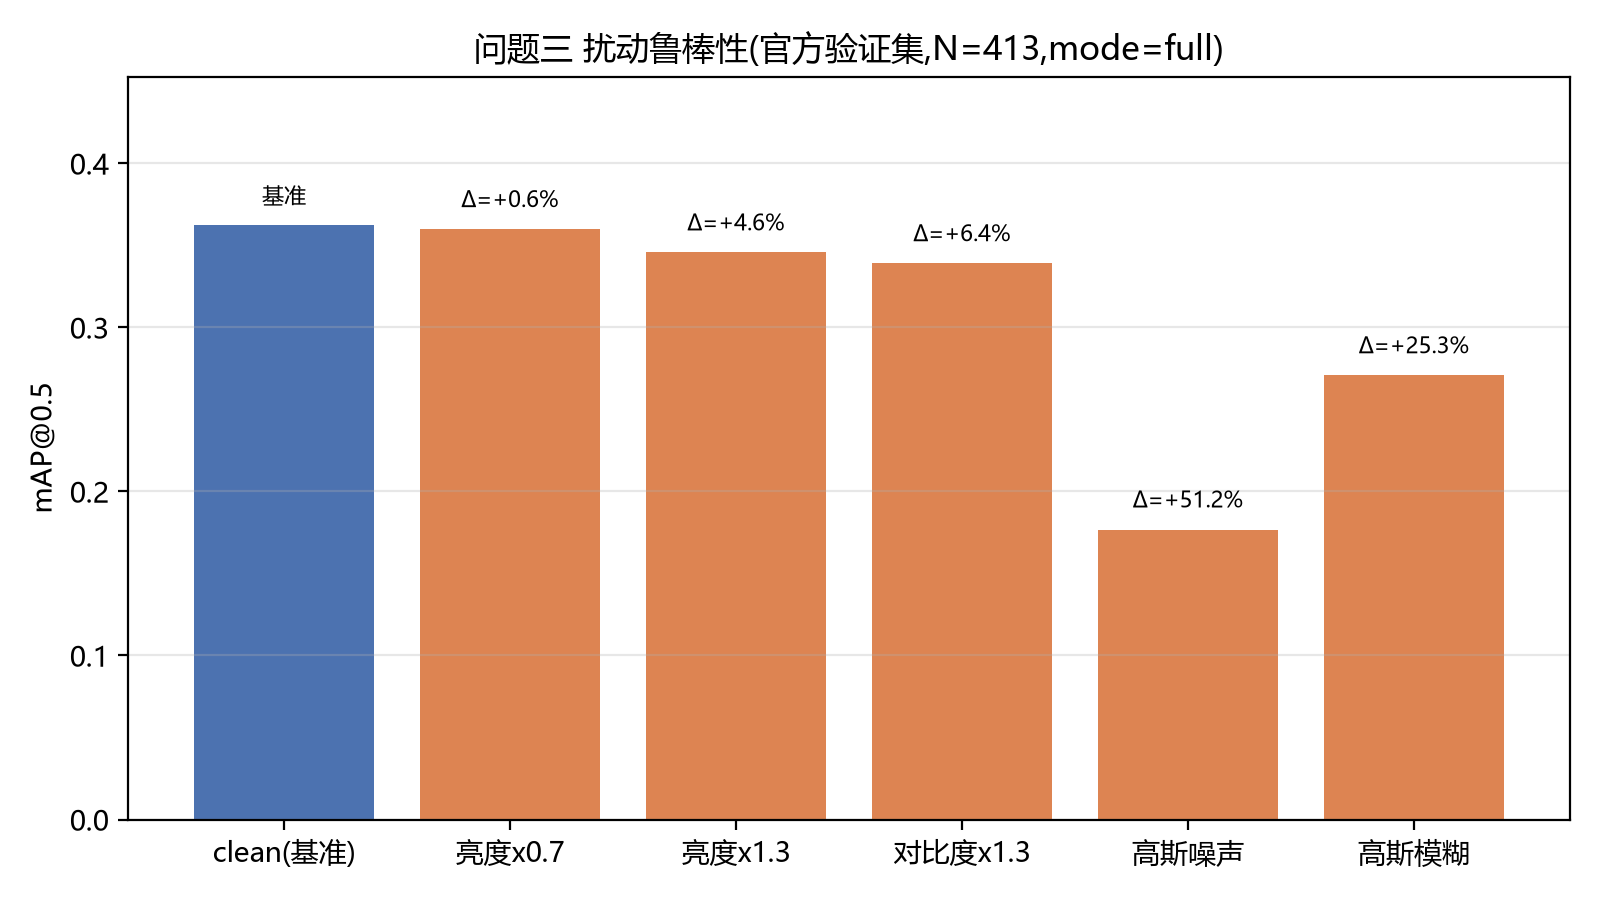
\includegraphics[width=0.85\textwidth]{figures/fig_q3_robust.png}
% \caption{各扰动下 mAP@0.5 衰减柱状图}
% \label{fig:q3-robust}
% \end{figure}
% \begin{figure}[h]
% \centering
% 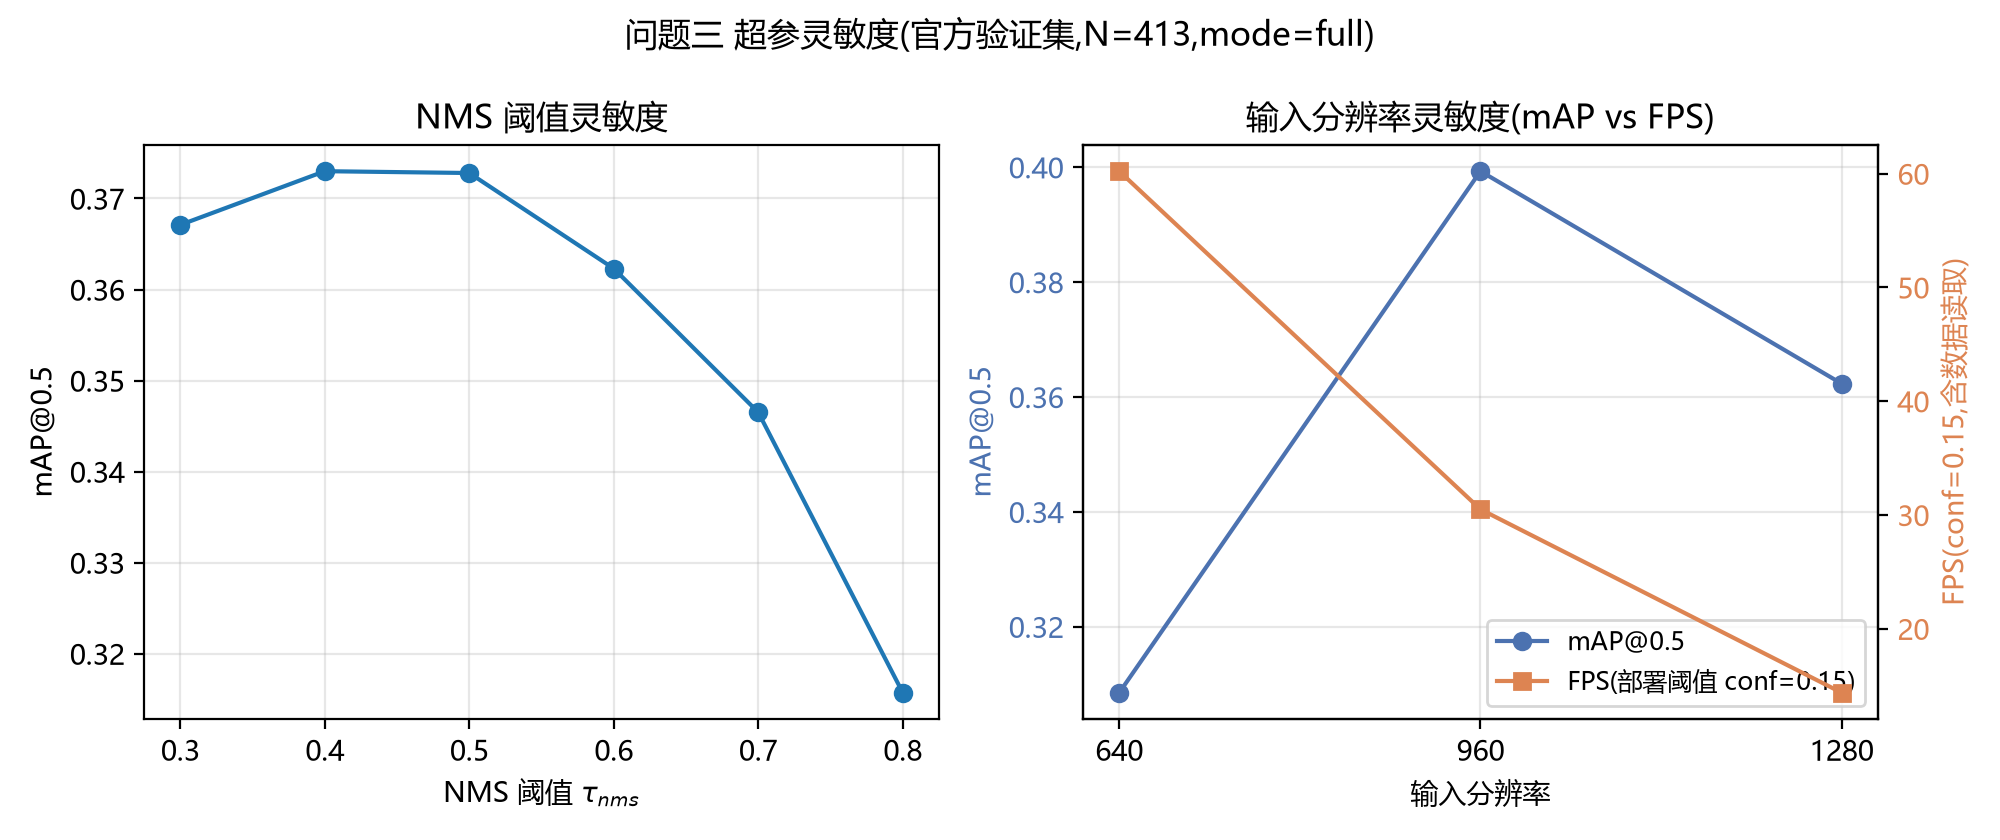
\includegraphics[width=0.95\textwidth]{figures/fig_q3_sens.png}
% \caption{超参灵敏度曲线(左:$\tau_{nms}$ 对 mAP;右:分辨率对 mAP/FPS)}
% \label{fig:q3-sens}
% \end{figure}
% \begin{figure}[h]
% \centering
% 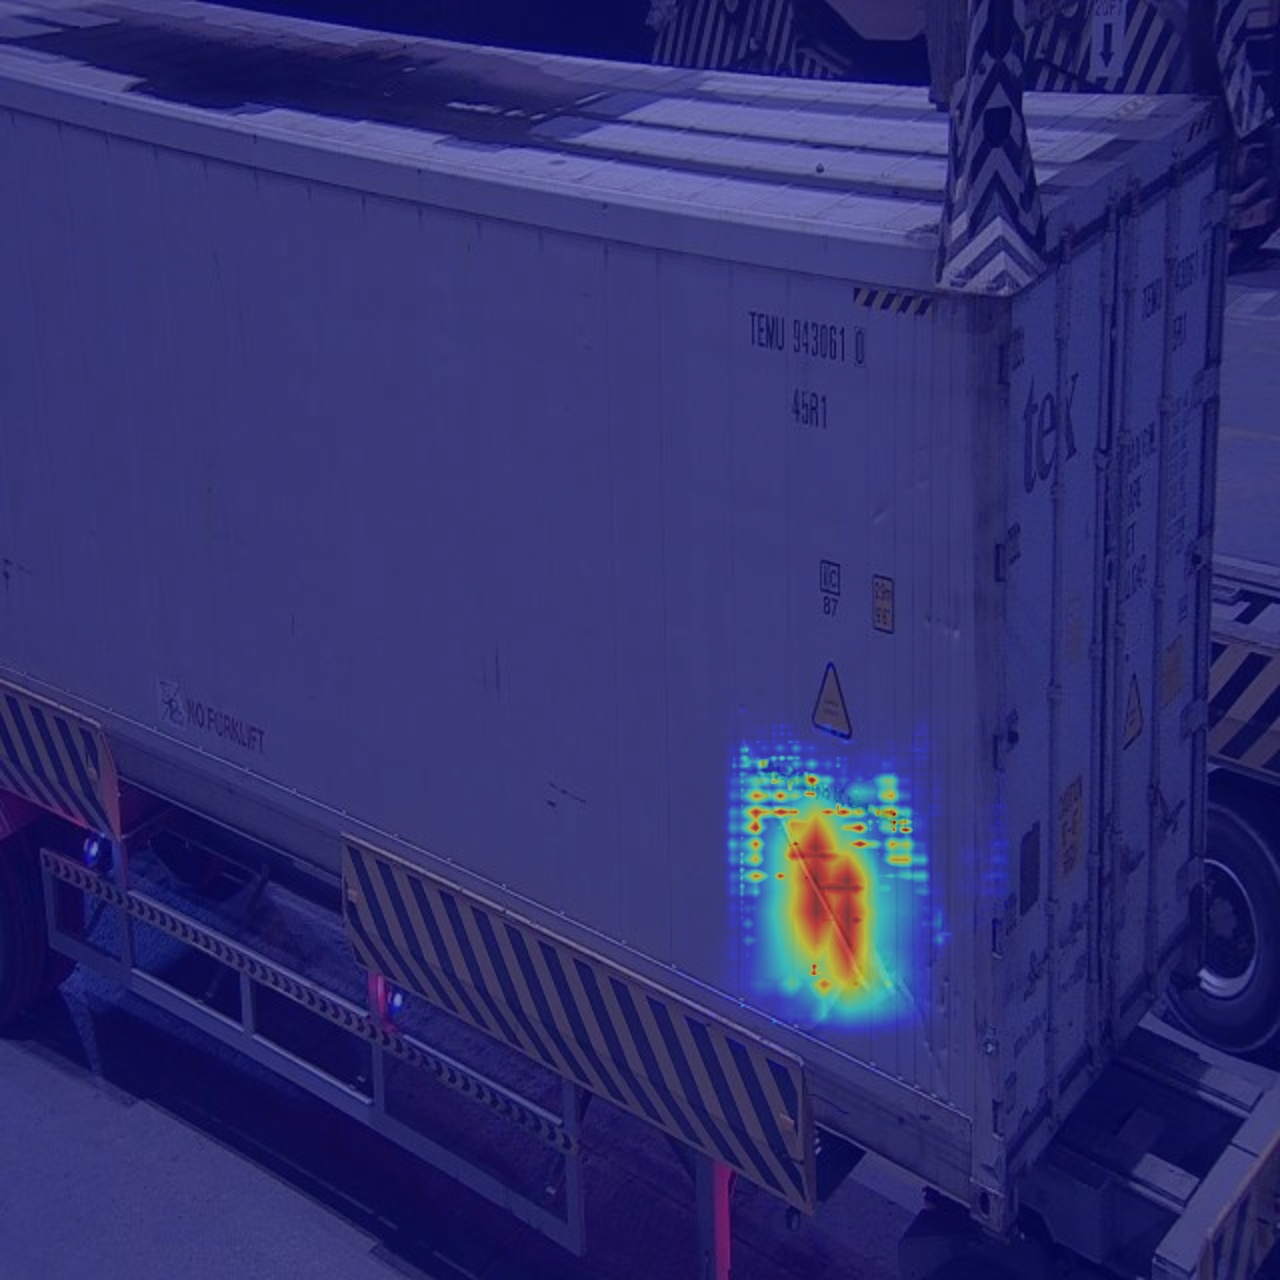
\includegraphics[width=0.32\textwidth]{figures/fig_q3_gradcam_Dent_1014.png}\hfill
% 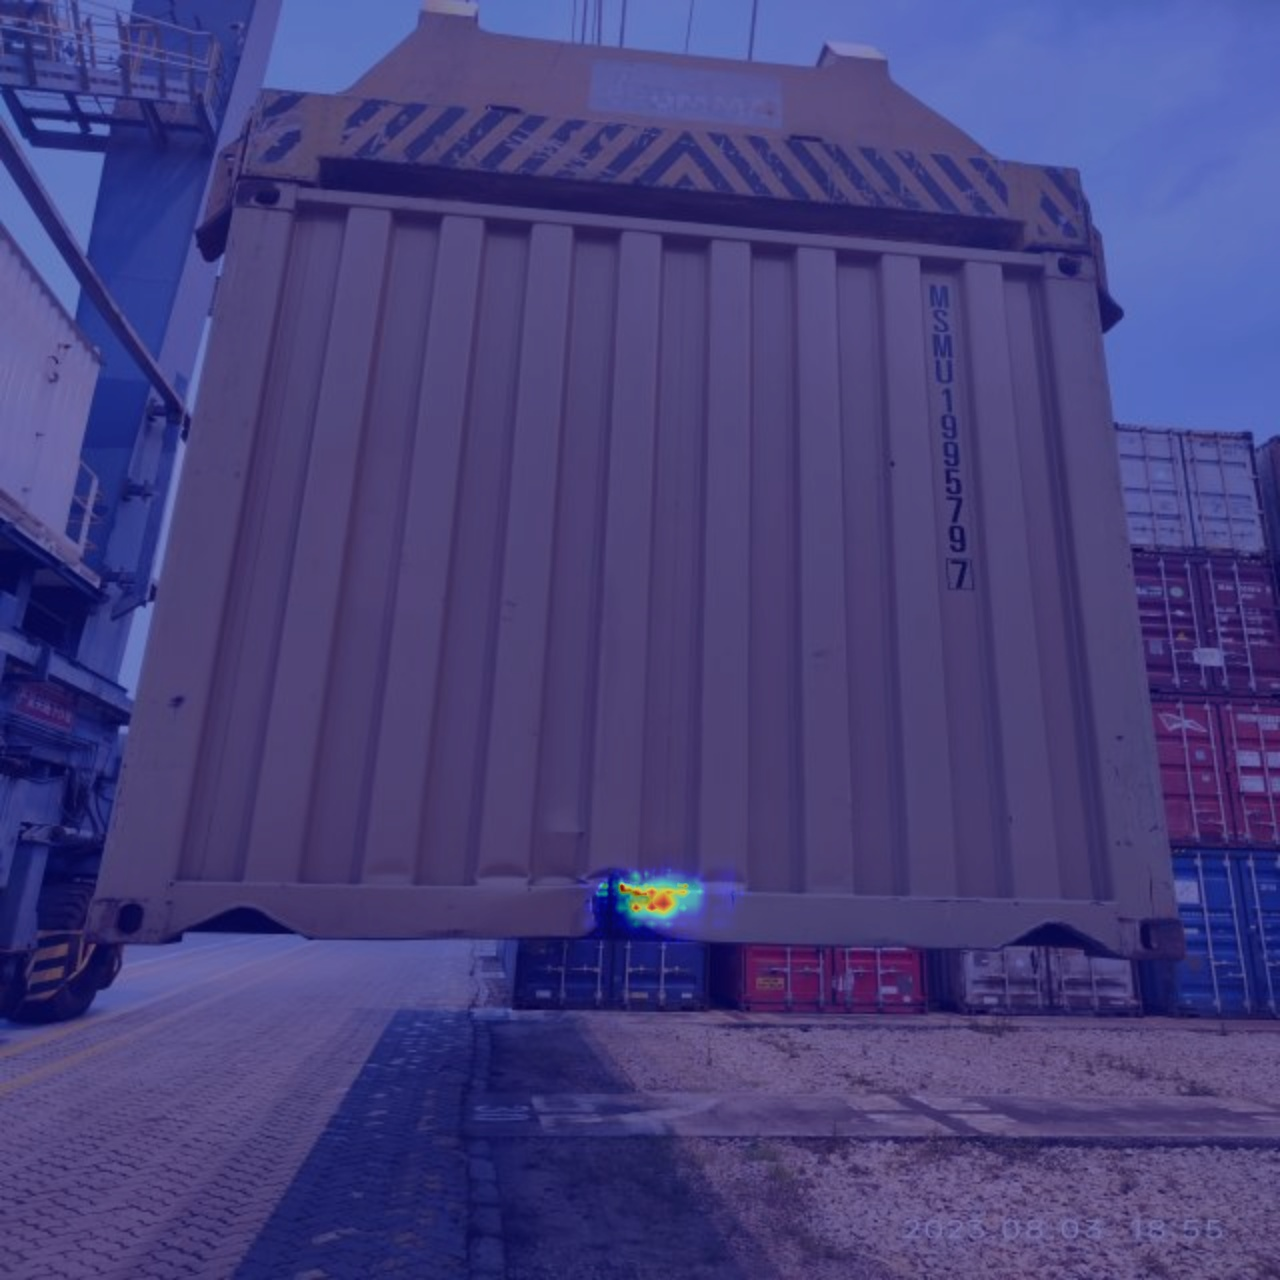
\includegraphics[width=0.32\textwidth]{figures/fig_q3_gradcam_Hole_1077.png}\hfill
% 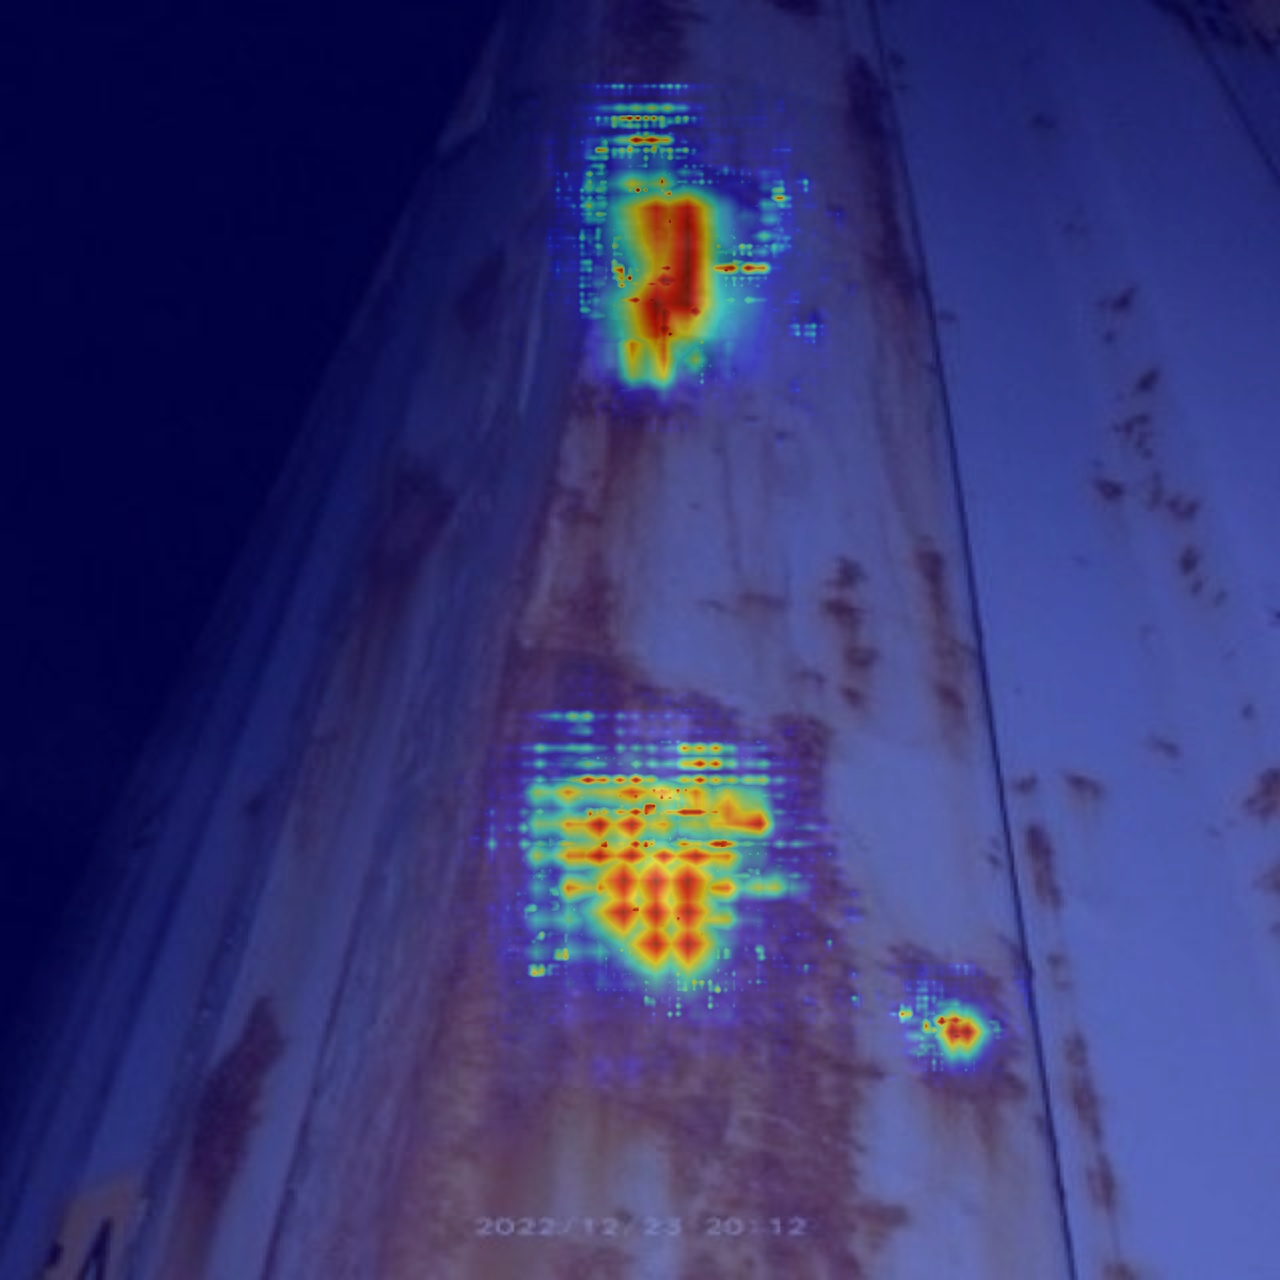
\includegraphics[width=0.32\textwidth]{figures/fig_q3_gradcam_Rusty_1.png}
% \caption{Grad-CAM 可视化样例(左起:凹陷/破洞/锈蚀各一例,热区=模型关注区域)}
% \label{fig:q3-gradcam}
% \end{figure}
